\begin{figure}[H]
	\centering
	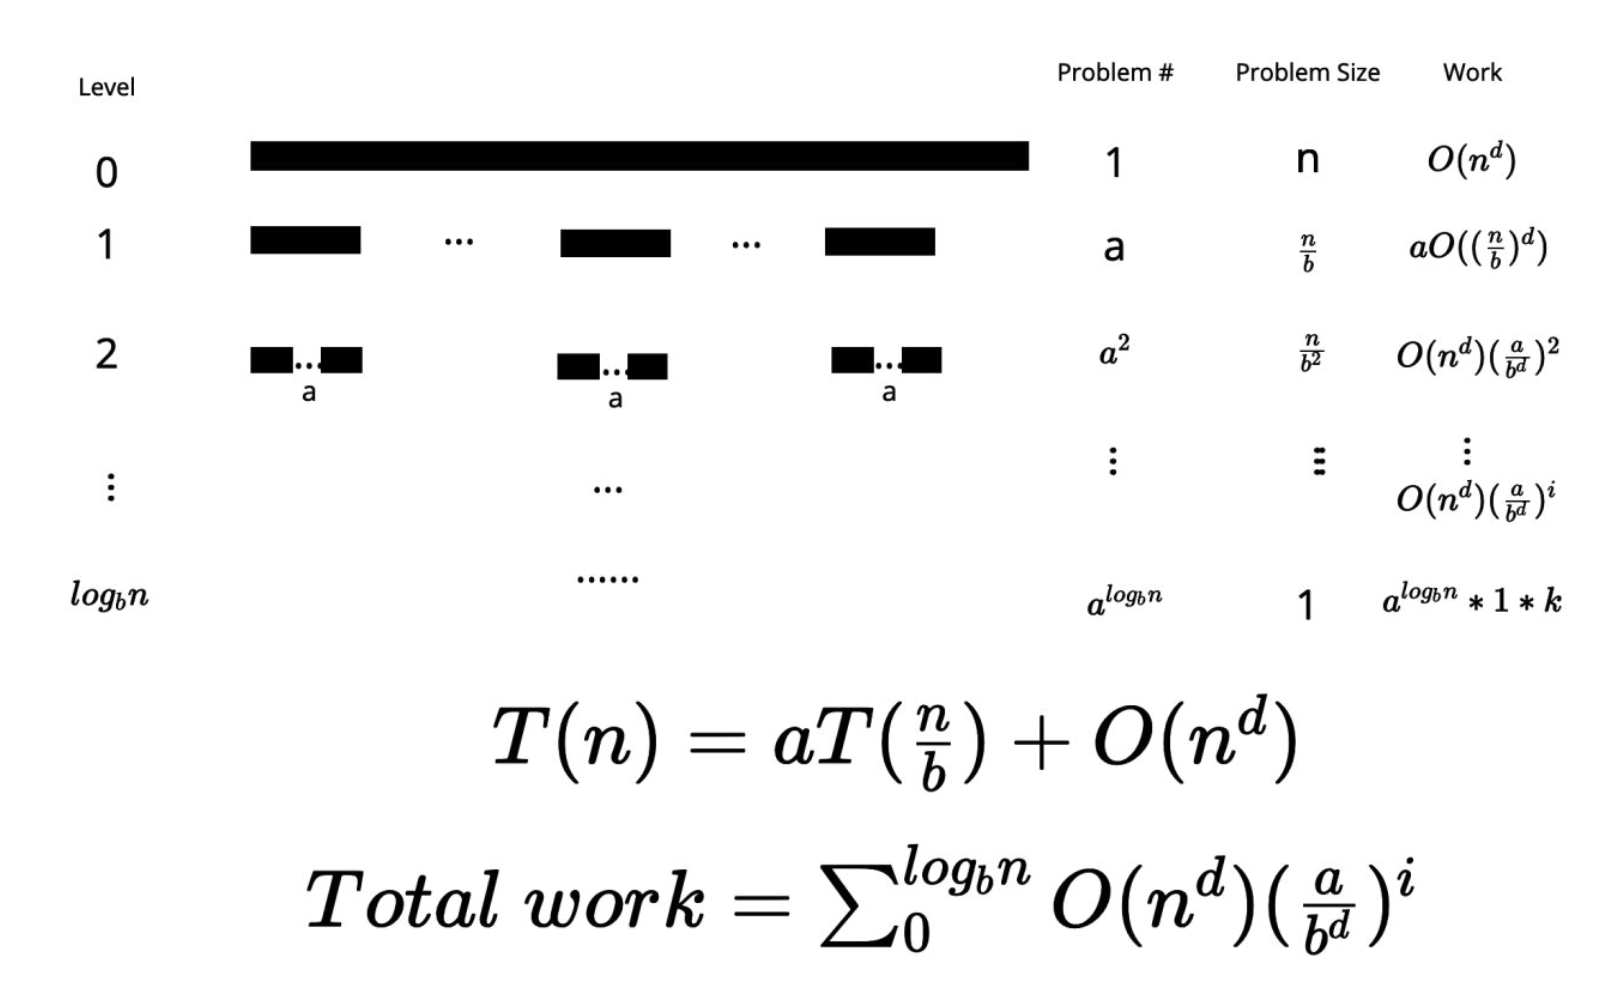
\includegraphics[width=0.8\textwidth]{master-method.png}
\end{figure}
%\begin{figure}[H]
%	\centering
%	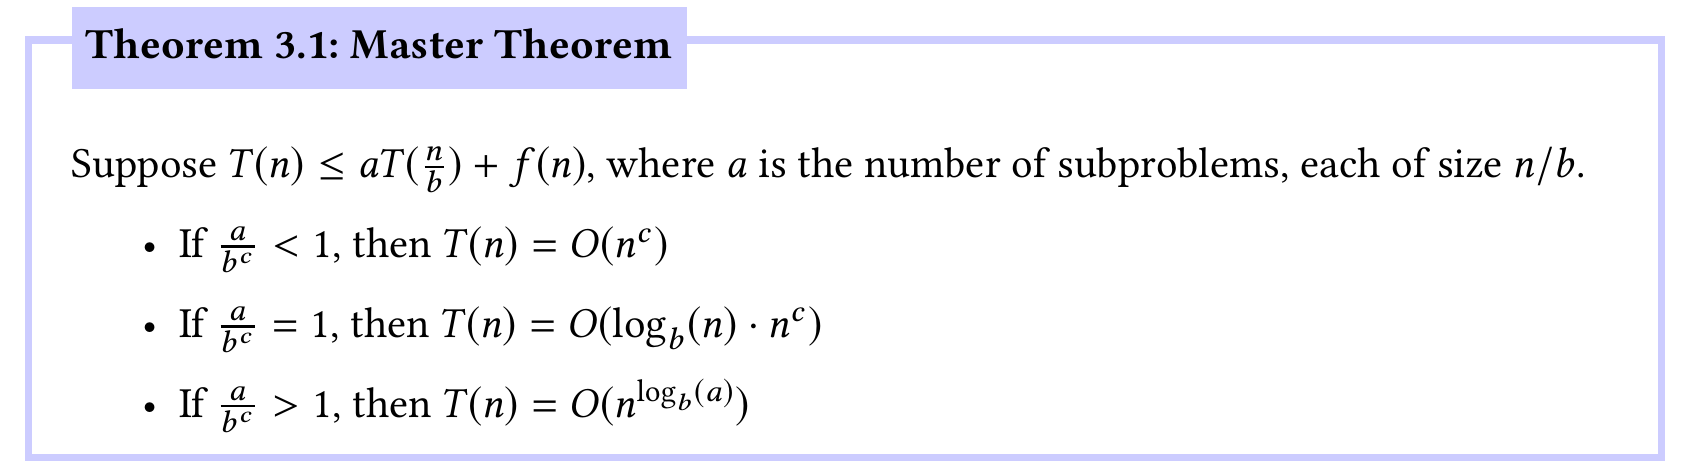
\includegraphics[width=0.5\textwidth]{master-method-2.png}
%\end{figure}
\begin{theorem}
	\textbf{Master Theorem:} Suppose $T(n) \le a T(\frac{n}{b}) + f(n)$, where $a$ is the number of subproblems, each of size $n / b$. Then
	\begin{itemize}
		\item If $\frac{n^c}{n^{\log_b a}} > 1$, the root dominate the running time, then $T(n) = O(n^c)$.
		\item If $\frac{n^c}{n^{\log_b a}} = 1$, intermidiate levels should be considered, then $T(n) = O(log_b n \cdot n^c)$.
		\item If $\frac{n^c}{n^{\log_b a}} < 1$, the leaves dominate the running time, then $T(n) = O(n^{\log_b a})$
	\end{itemize}
\end{theorem}